\section{Prototype \#3}
\label{sec:implementation:prototypes:prototype3}

The purpose of the third prototype, 
was to test indoor positioning using the Estimote beacons, 
as well as test the use of gesture recognition on a smartphone.

\subsection{Description}
The third prototype builds upon the second prototype for iOS, 
which was expanded to include some new features. 
The second prototype would assume that the user was positioned in the center of the room, 
but the new prototype takes the users position into account when determining devices being pointed at. 
Estimote beacons and the SDK provided by Estimote for indoor positioning was utilized, 
in order to determine the position of the user.

The indoor SDK from Estimote provides a visualization of the room, 
in which the positioning takes place, 
as well as a visualization of the installed beacons, 
and the position of the user. 
The view can be used to visualize custom objects. 
\Cref{fig:prototype3-room-screenshot} shows two red circles in the room. 
Each of the circles represent one of the virtual lamps introduced in the second prototype. 
The color of the lamp indicates the state the lamp is in. 
A lamp can either be on or off. 
The states are represented by green and red respectively.

Furthermore the prototype added support for training and recognizing gestures, 
using the \threedollar library described in \Cref{sec:threedollar}.
Users can add a gesture by giving the gesture a name, 
and train it at least \num{5} times. 
When added, the gesture can be used when pointing at a lamp, 
to toggle the state of the lamp. 
For example, if the user has trained a circle named ``Half Circle'', 
he can visit the screen showing his lamps and his position, 
point at one or more lamps and perform the ``Half Circle'' gesture, 
in order to either turn on or turn off the lamps.

The third prototype does not support associating a gesture with an action, 
\ie performing a specific action for a specific gesture. 
Nor does it support creating a model of a room. 
The prototype is limited to a specific (hardcoded) room,
modeled after the living room of one of the research members.

\subsection{Major Changes}
\begin{itemize}
\item Uses BLE beacons to position the user in a room, and take his position into account, when determining devices being pointed at.
\item Adds training and recognition of gestures, in order to trigger actions of a controllable device.
\item Adds a graphical representation of the room, in which the beacons and the devices are installed.
\end{itemize}

\subsection{Results}

We were able to get the position of the user by using Estimote beacons, 
allowing the application to keep track of the user. 
In addition, the \threedollar library was introduced, 
which allows users to control the lamps by performing a gesture with the phone.
The accuracy of Estimote is explored in \Cref{sec:estimoteprecision}, 
and the performance of the gesture recognition is explored in \Cref{sec:gestureperformance}.

The prototyped used simulated devices, 
and the next step is to control actual smart devices, 
and give the user a more fine grained control, 
over which devices are controlled when preforming a gesture.

\begin{figure}[!htb]%
    \centering
    \subfloat{
        \frame{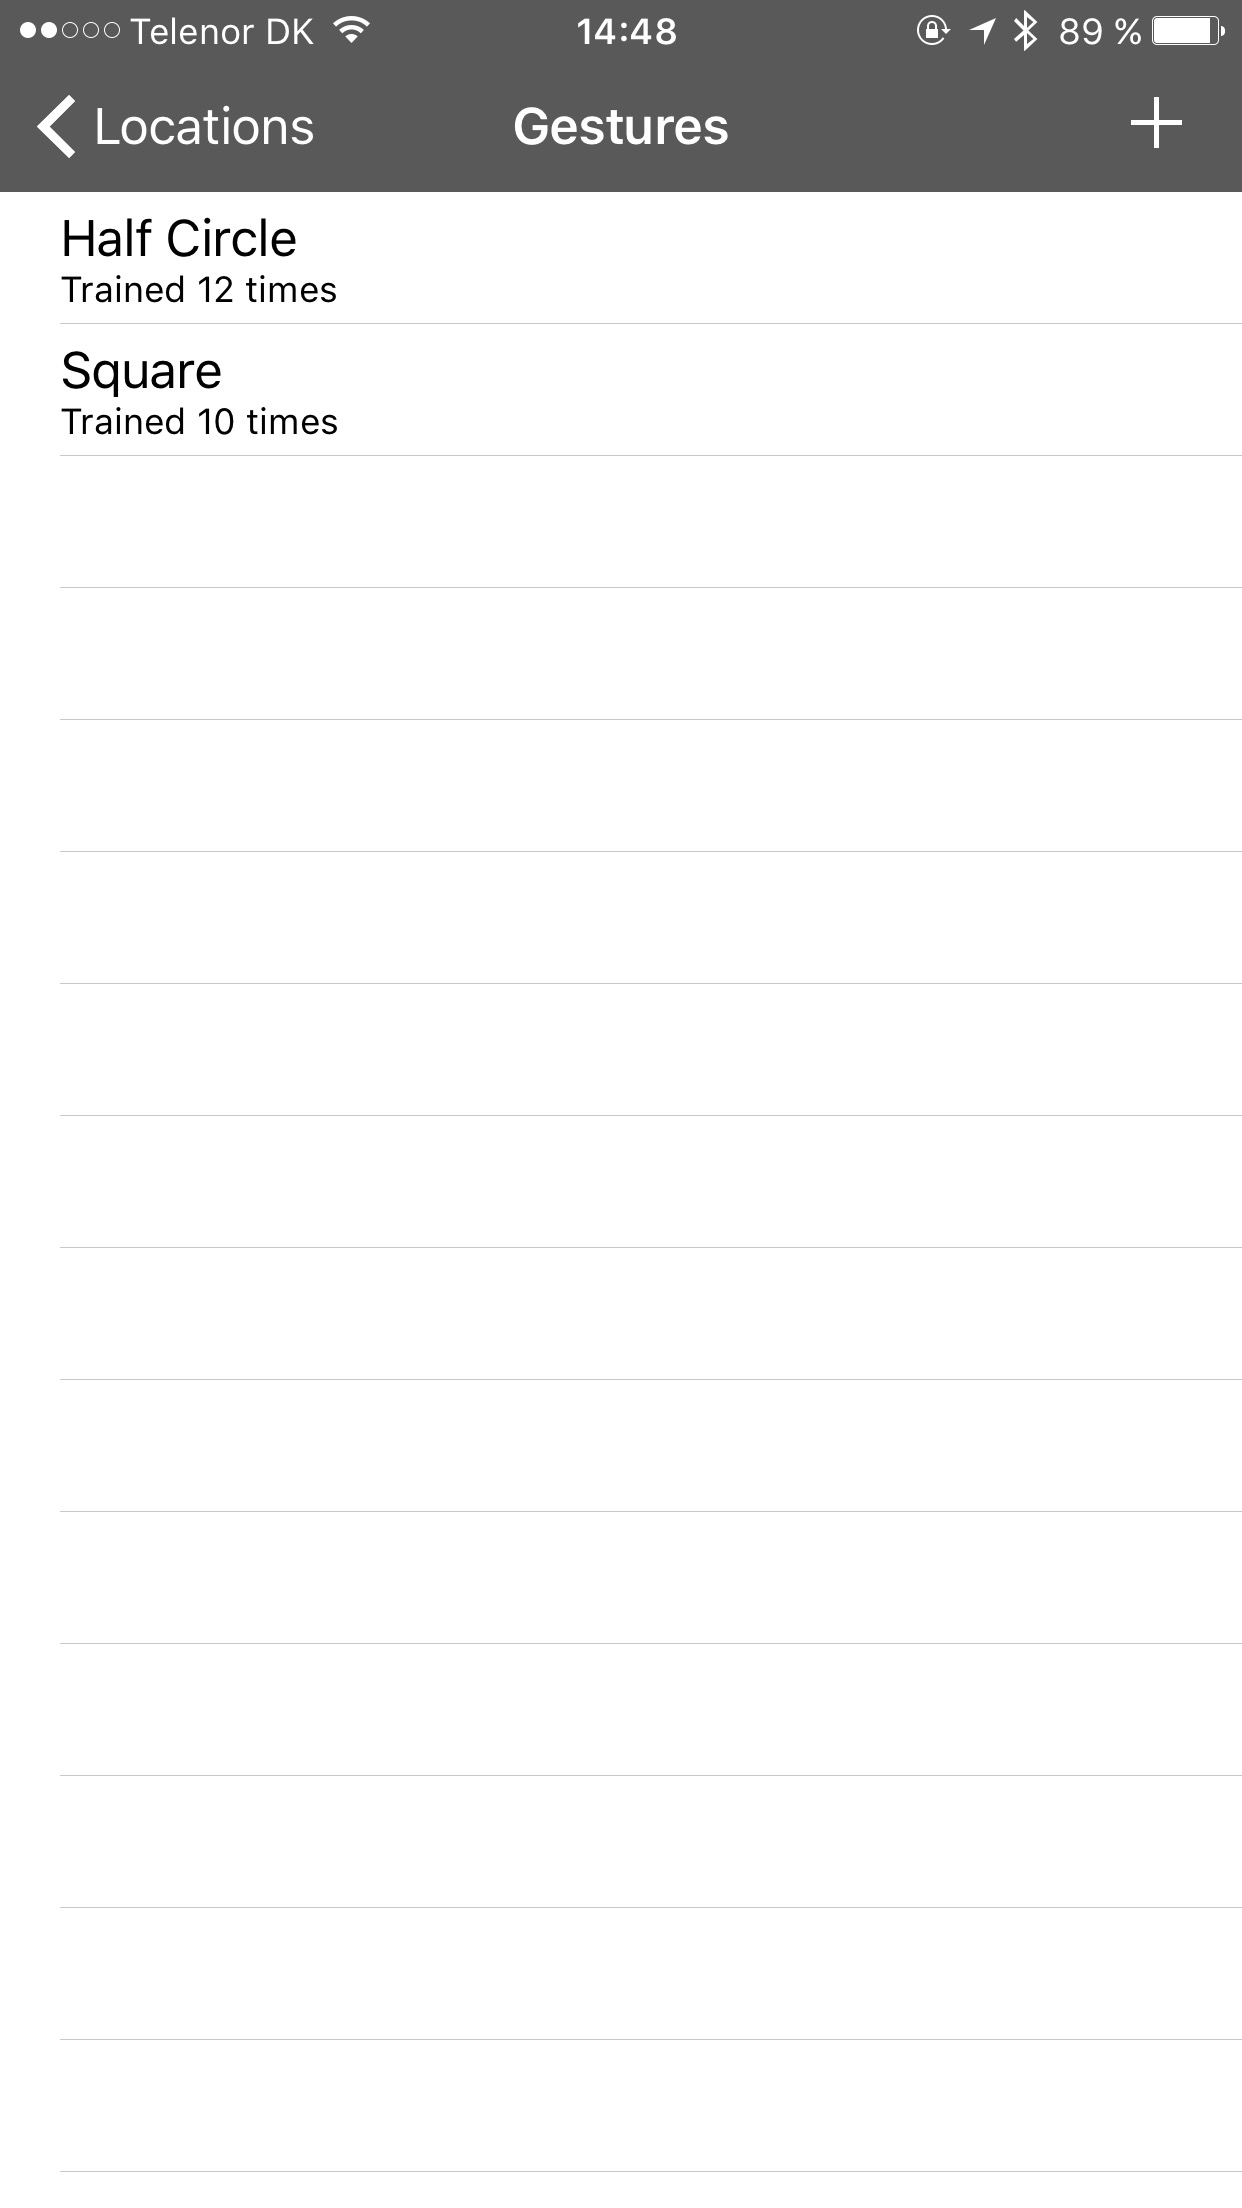
\includegraphics[width=0.3\textwidth]{images/prototype-3-all-gestures}}
    }
    \subfloat{
        \frame{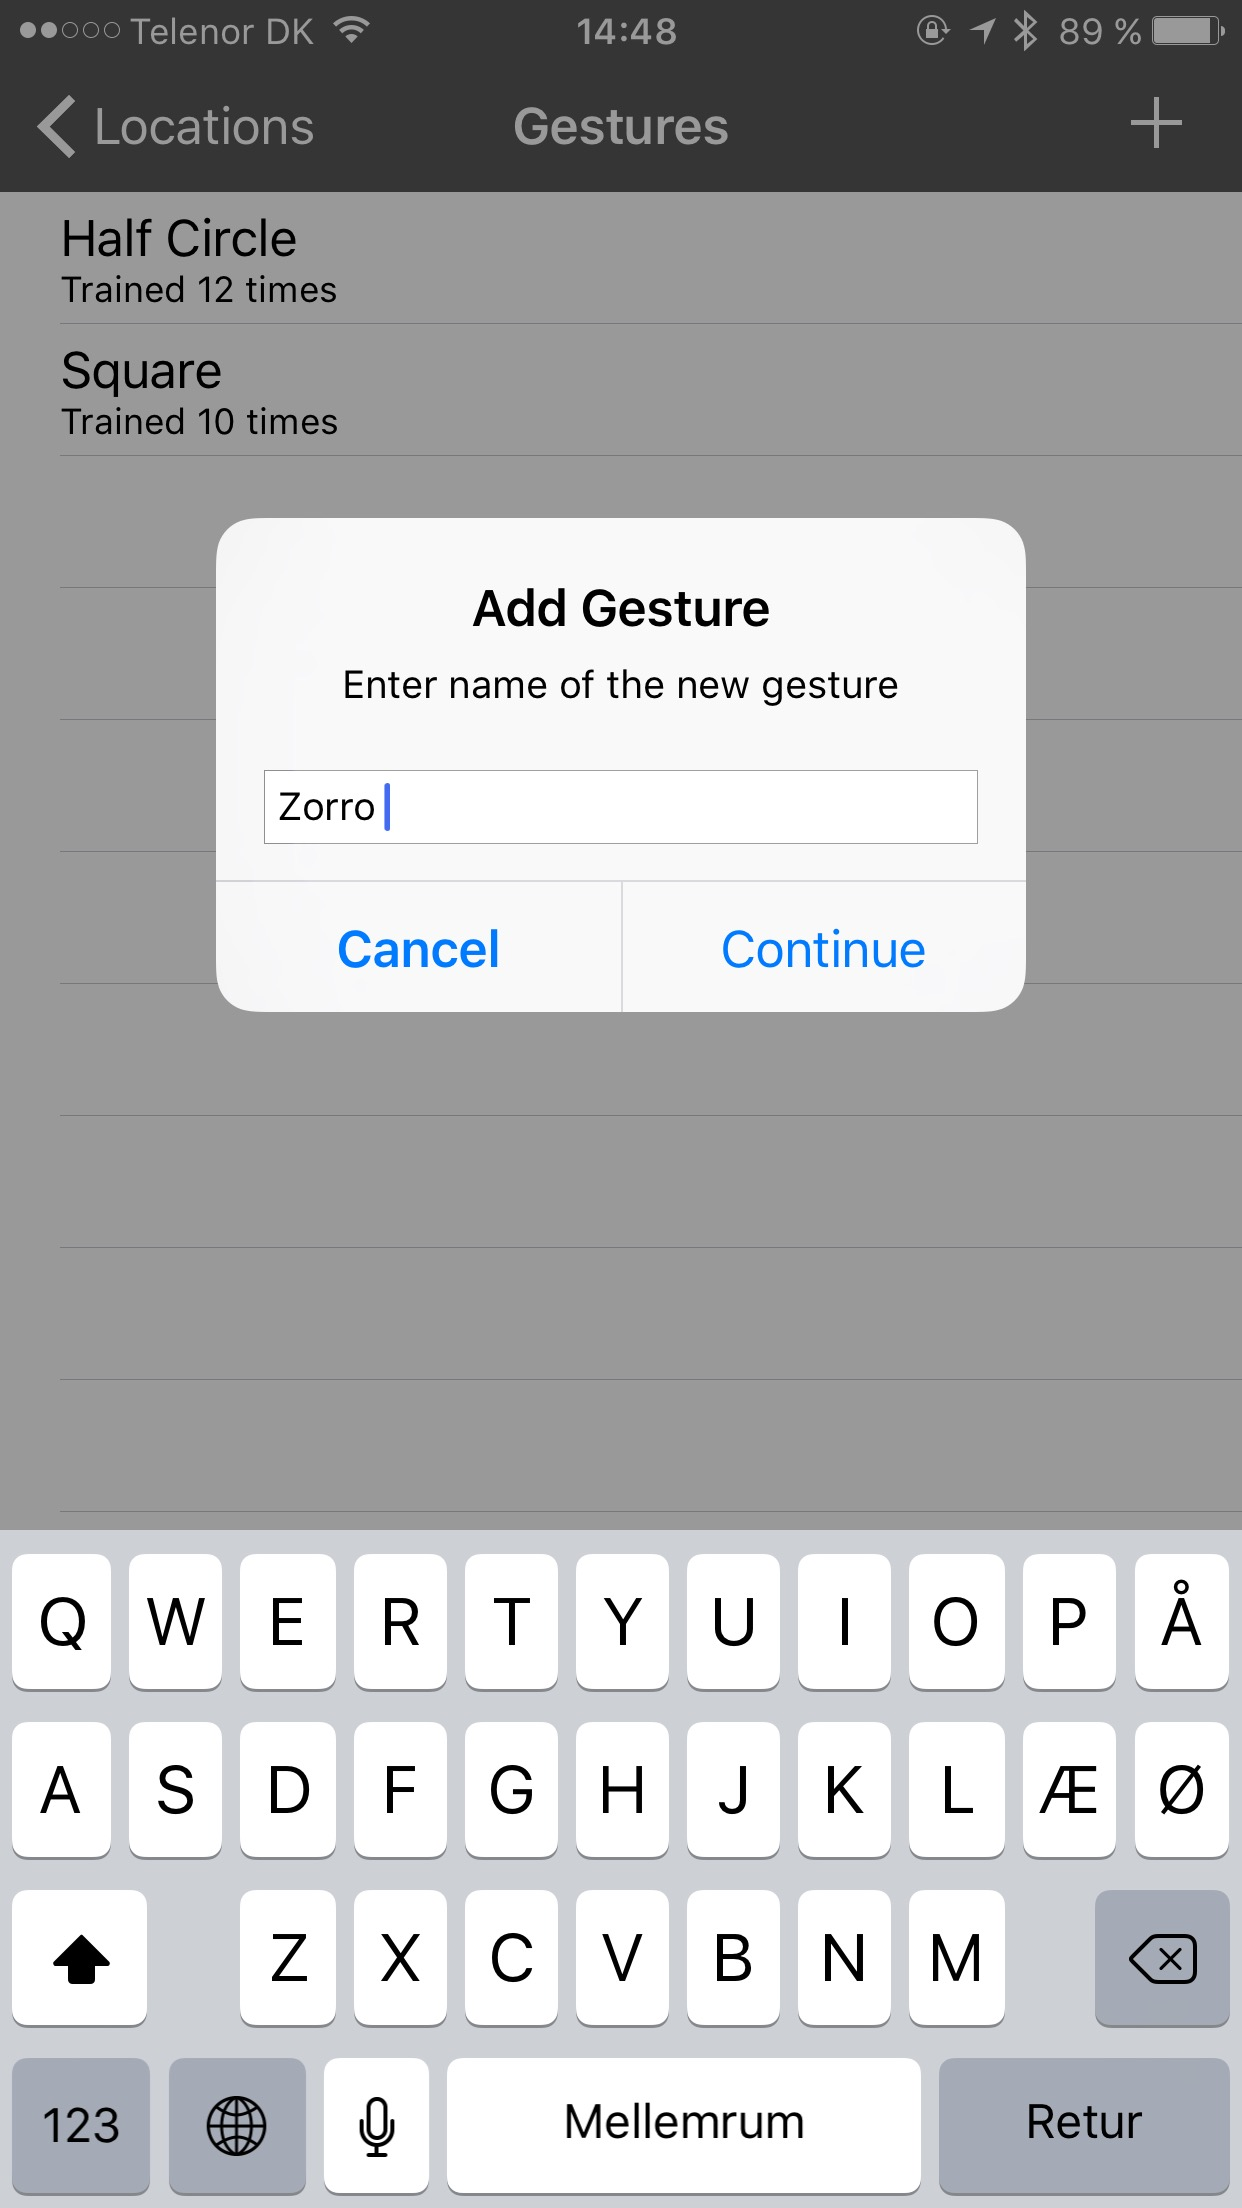
\includegraphics[width=0.3\textwidth]{images/prototype-3-new-gesture}}
    }
    \subfloat{
        \frame{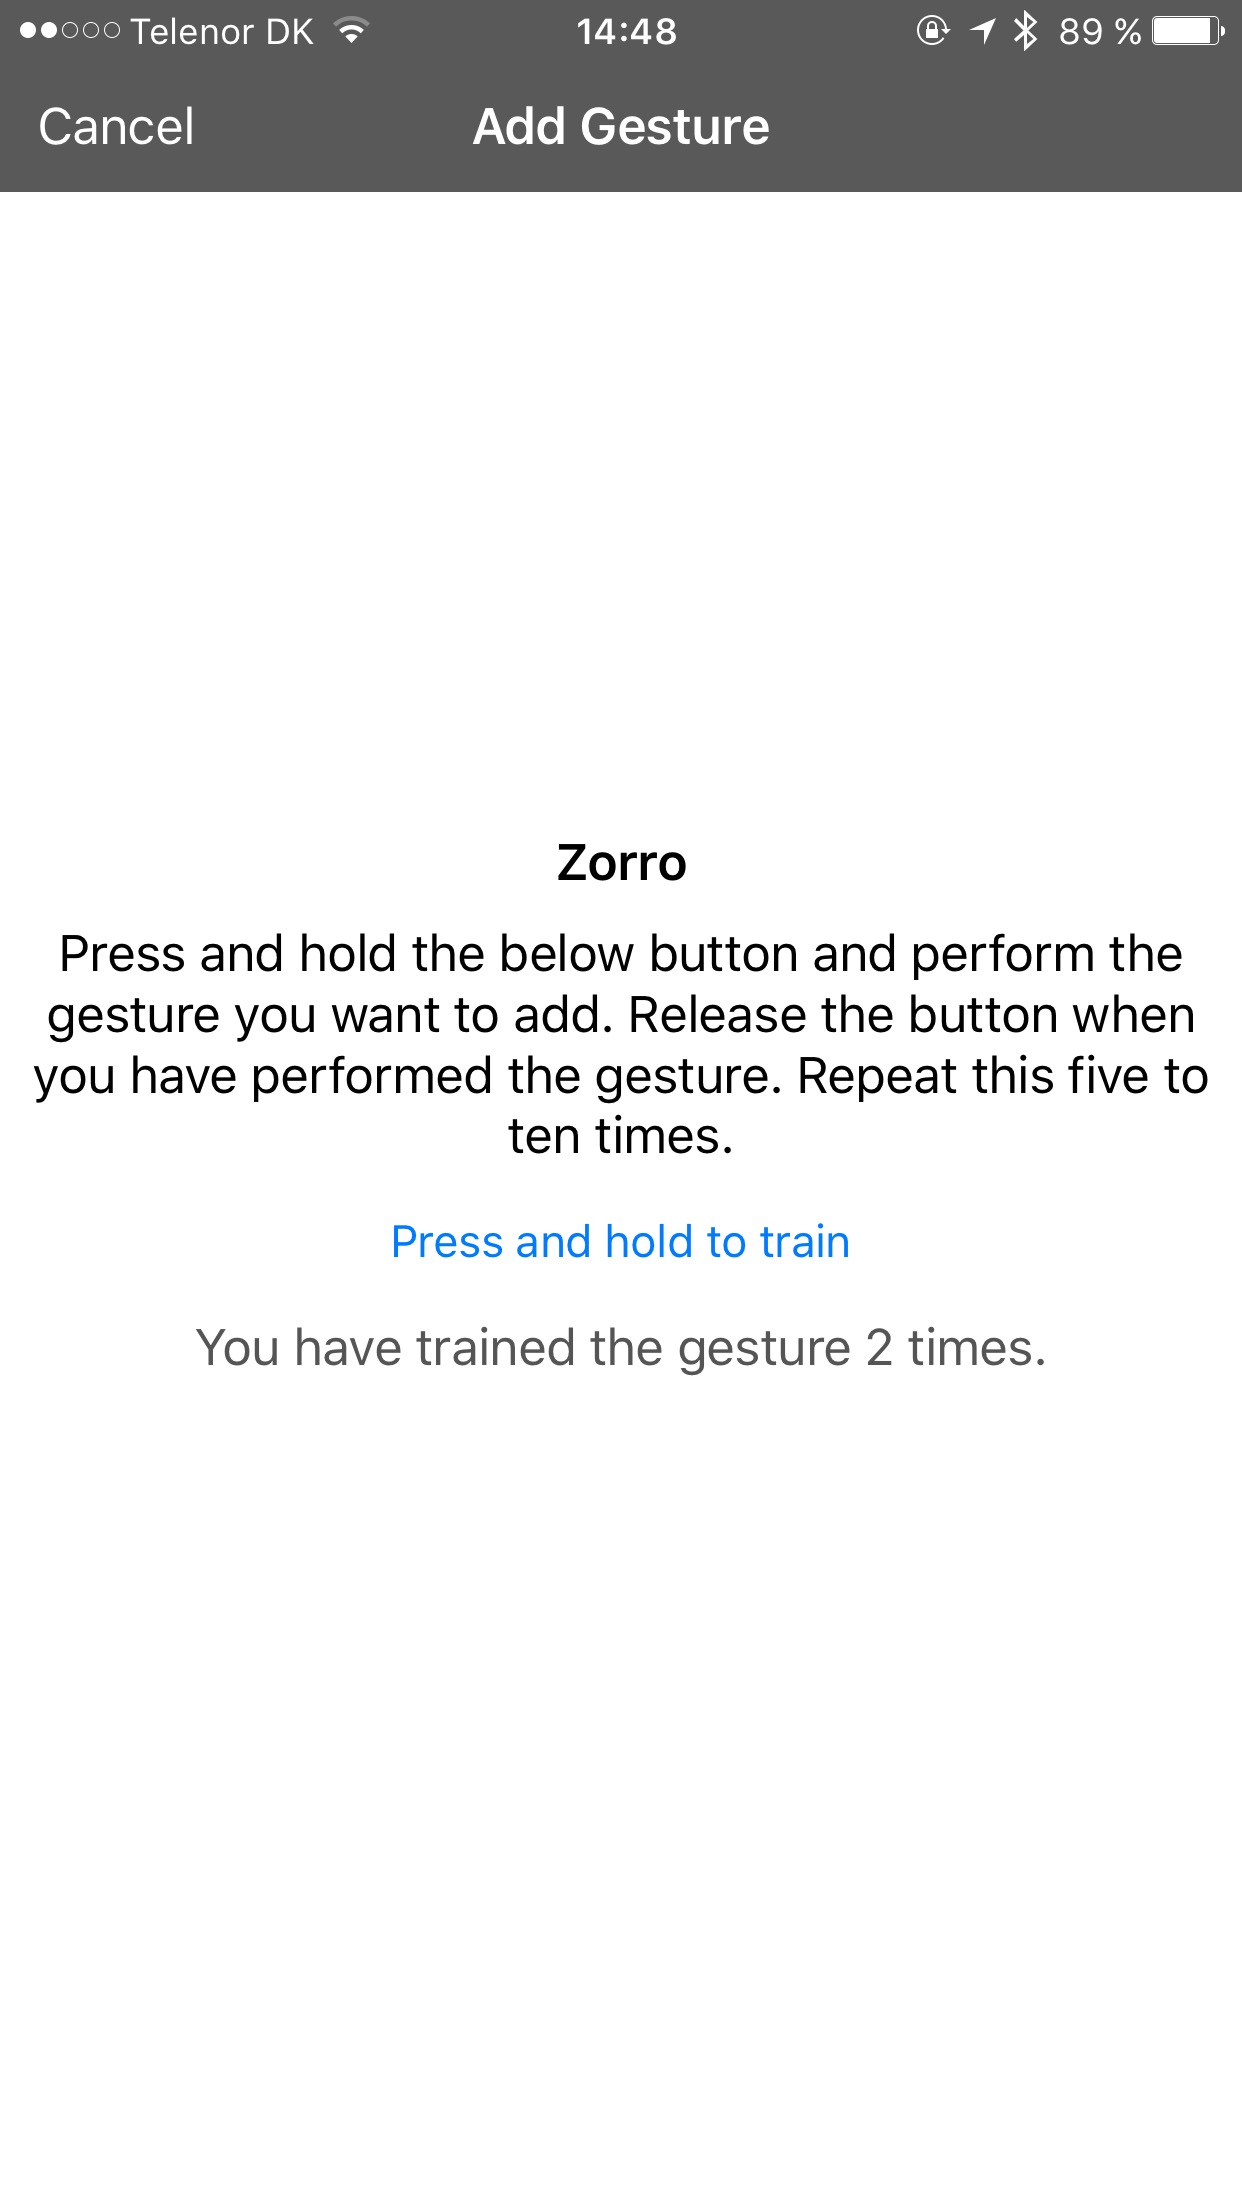
\includegraphics[width=0.3\textwidth]{images/prototype-3-train-gesture}}
    }
    \caption{Screenshots showing the flow and interface for adding and training a new gesture in the third prototype.}
    \label{fig:prototype3-gesture-screenshots}
\end{figure}

\begin{figure}[!htb]%
    \centering
    \frame{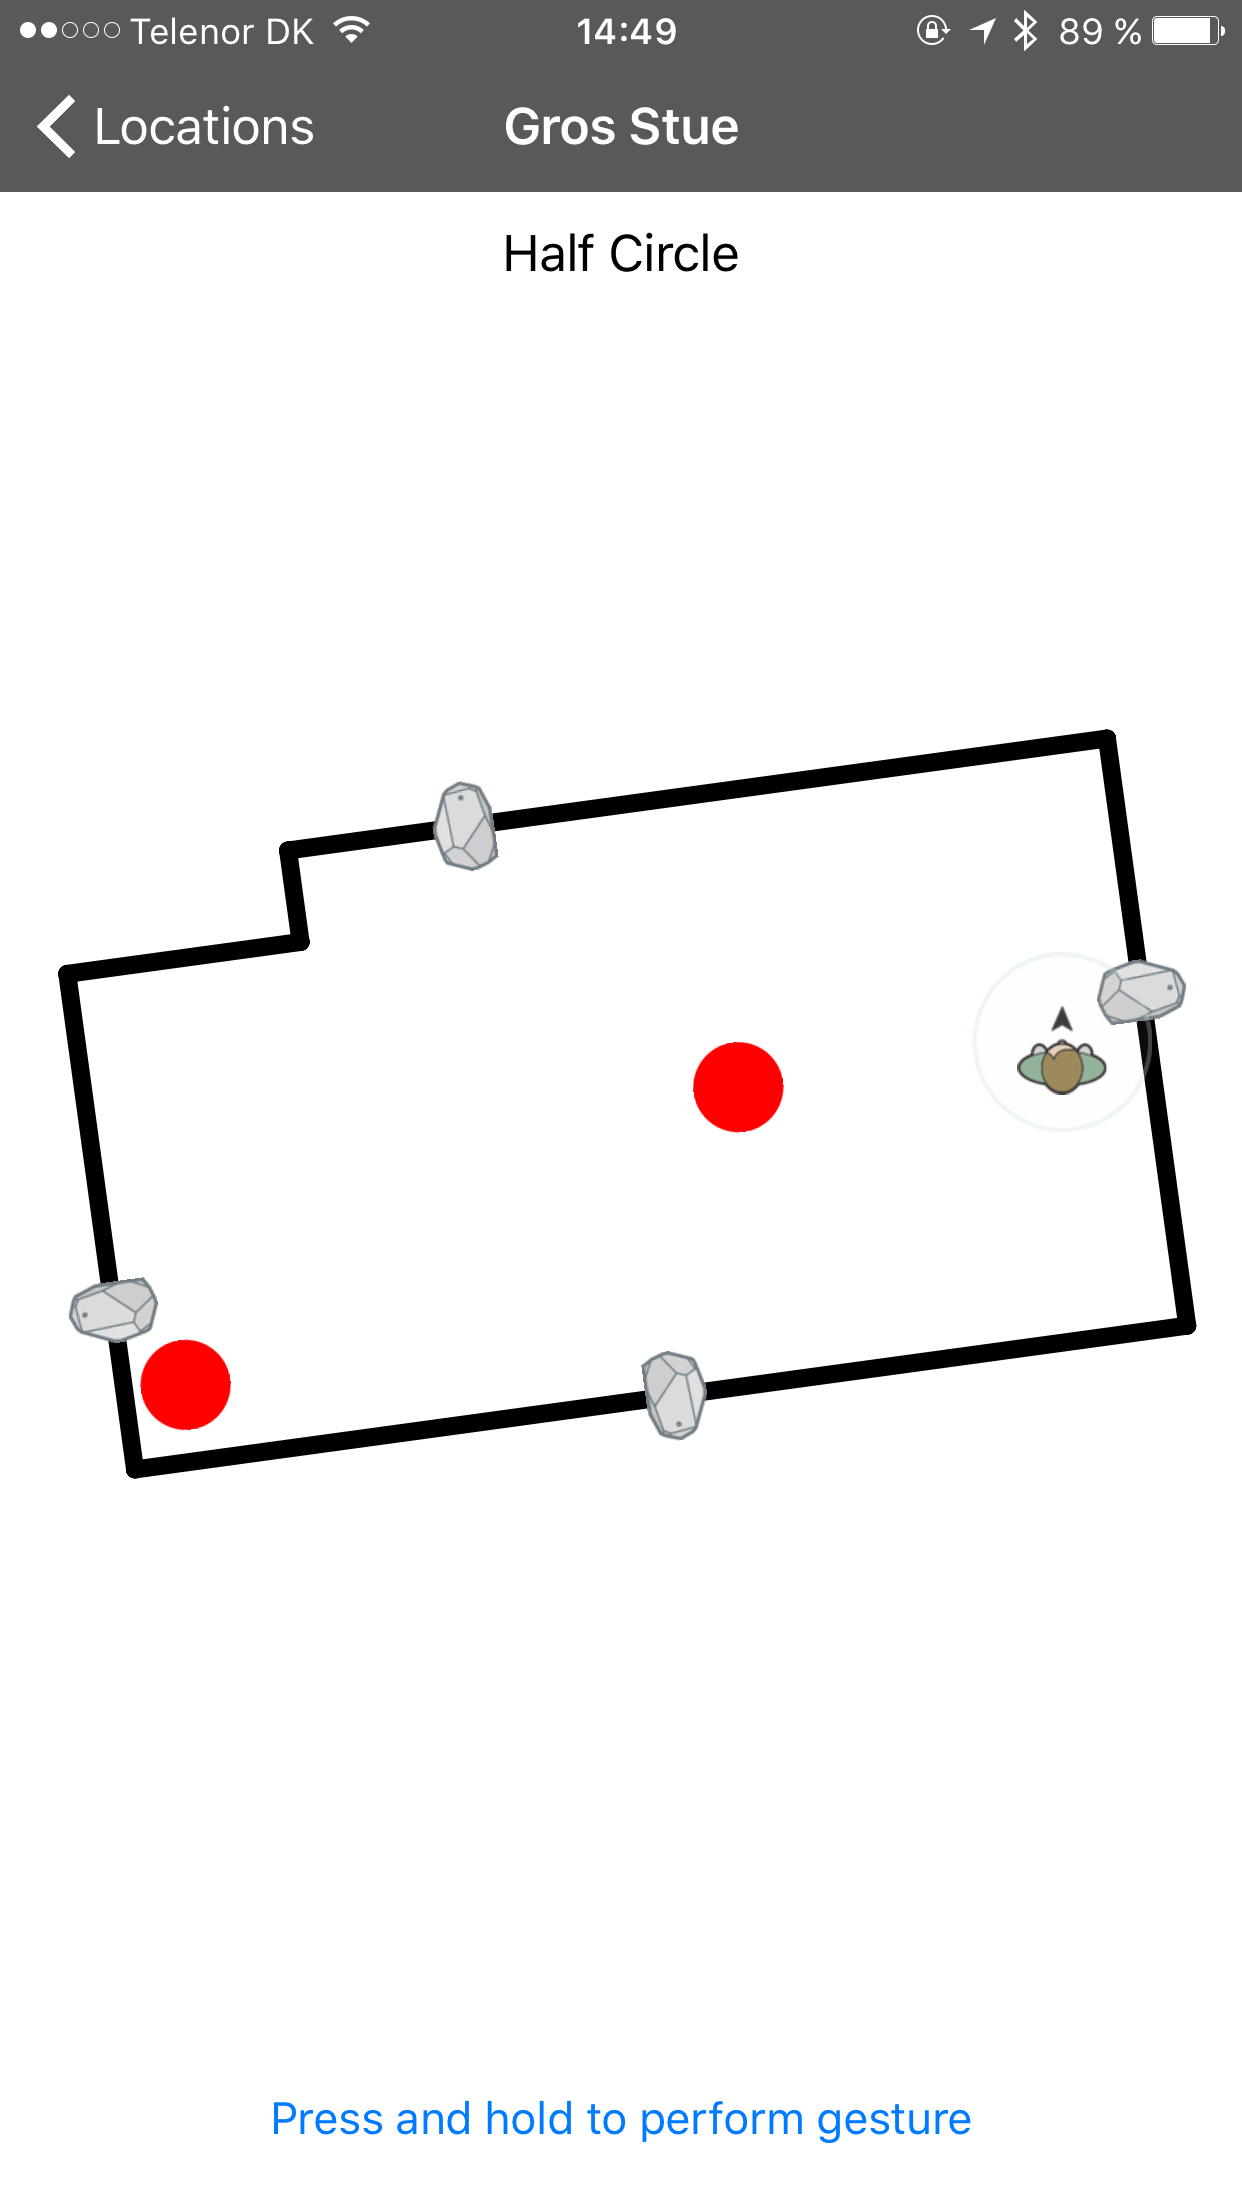
\includegraphics[width=0.3\textwidth]{images/prototype-3-gesture-triggered}}
    \caption{Screenshot showing new representation of the room and controllable devices. In this screenshot the gesture named ``Half Circle'' was recently recognized, and therefore the gesture name is shown in the top of the screen.}
    \label{fig:prototype3-room-screenshot}
\end{figure}

%%% Local Variables:
%%% mode: latex
%%% TeX-master: "../../master"
%%% End:
